\documentclass[14pt]{matmex-diploma-custom}
\linespread{1.5}
\usepackage{listings}
\usepackage{cite}

\usepackage{framed}
\usepackage{tikz}
\usetikzlibrary{arrows}
\usepackage{amssymb}
\newcommand{\cd}[1]{\texttt{#1}}
\usepackage[caption=false]{subfig}
\usepackage{lstcoq}
\graphicspath{{images/}}%путь к рисункам

\lstdefinelanguage{haskell}{
keywords={data, type, case, of, where, otherwise, in, let, deriving},
sensitive=true,
basicstyle=\small,
commentstyle=\scriptsize\rmfamily,
keywordstyle=\ttfamily\underbar,
identifierstyle=\ttfamily,
basewidth={0.5em,0.5em},
columns=fixed,
fontadjust=true,
literate={->}{{$\to$}}1
}

\lstset{
basicstyle=\small,
identifierstyle=\ttfamily,
keywordstyle=\bfseries,
commentstyle=\scriptsize\rmfamily,
basewidth={0.5em,0.5em},
fontadjust=true,
escapechar=~,
language=haskell
}
%\DeclareMathSizes{16}{16}{16}{16}
\definecolor{dkviolet}{RGB}{100,0,100}
\definecolor{ltblue}{RGB}{0,100,100}
\definecolor{dkblue}{RGB}{0,50,50}

\begin{document}

\filltitle{ru}{
    chair              = {Кафедра Системного Программирования},
    title              = {История язков ML},
    author             = {ИЗМЕНИТЬ ИЗМЕНИТЬ ИЗМЕНИТЬ },
    supervisorPosition = {к.\,ф.-м.\,н.},
    supervisor         = {Терехов А.\,Н.},
}
\sloppy

%\maketitle
%\tableofcontents

\newpage
\section*{Введение}

\setlength{\unitlength}{1mm}
\begin{picture}(160, 40)
\put(20,30){\circle{1}}
\put(20,30){\circle{8}}
\put(20,30){\circle{16}}
\put(20,30){\circle{32}}

\put(25,10){\circle*{3}}
\put(30,10){\circle*{4}}
\put(35,10){\circle*{5}}
\put(0,40){Max Newman}
\put(10,30){Alan Turing}
\put(20,20){Christopher Stratchey}
\put(50,40){Marvyn Pragnell}
\put(40,10){Peter Landin}
\put(90,20){Rod Burstall}
\put(2,3){\oval(13,5)}
\end{picture}
\newpage
\begin{center}


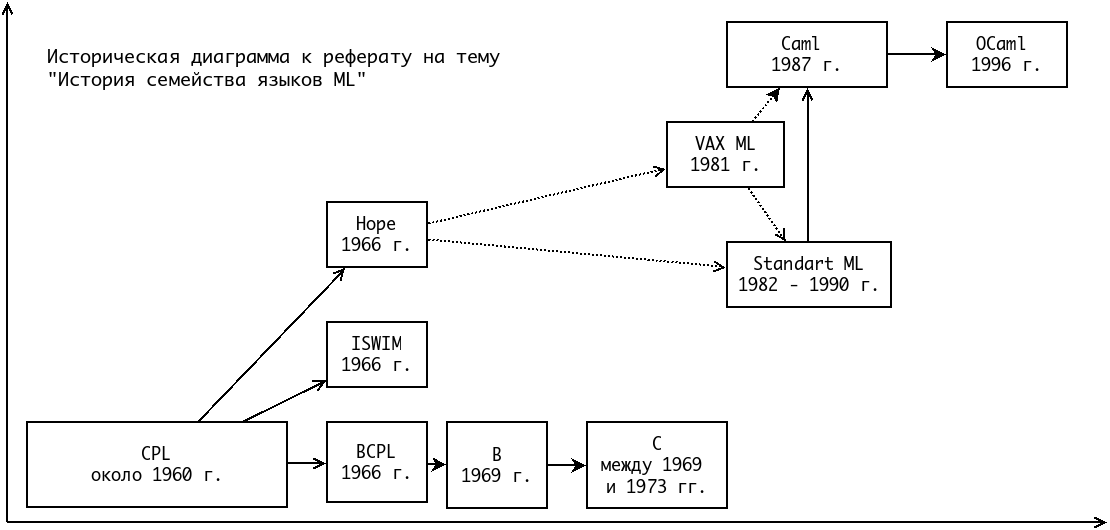
\includegraphics[angle=90,scale=0.585]{Diagram.png}
\end{center}

Британские исследователи языков програмирования

КАРТИНКА
Макс Ньюман, Алан Тьюринг, Кристофер Стрэтчи, Петер Лондин, Код Бёрсталл и Марвин Прагнелл
Стрэтчи был лидером  (но тут бла бла бла)

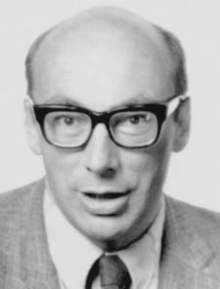
\includegraphics[angle=0,scale=0.585]{220px-Peter_Landin.png}
История про Прэгнелла и о том как он познакомился в кафе с Лондиным и книгой Principia Mathematica. Неформальная группа читателей книг. 
\begin{framed}
Бёрсталл впоминает как спросил человека рядом в библиотеке про какую-то книгу, гно
\end{framed}

Так вот, семинар был Бёркберк колледже без разрешения руководителей колледжа. Прэгнелл нашел человека с ключом , который их впустит, где они заседали до позднего вечера. Вместе  со Стрэтчи, Лондиным и Бёрсталом туда заходил и Робин Милнер. Там они обсуждали вопросы логинки, теории категорий и кмпьютеров. Это вероятно первый раз когда они все встретились.” Так получился первый любительский undergreound семинар и компьютерах. Для рассказчика запомнилось как по-любительски всё было устроено, в отличие от того как это было сделано в штатах. И они были работающими пограммистами

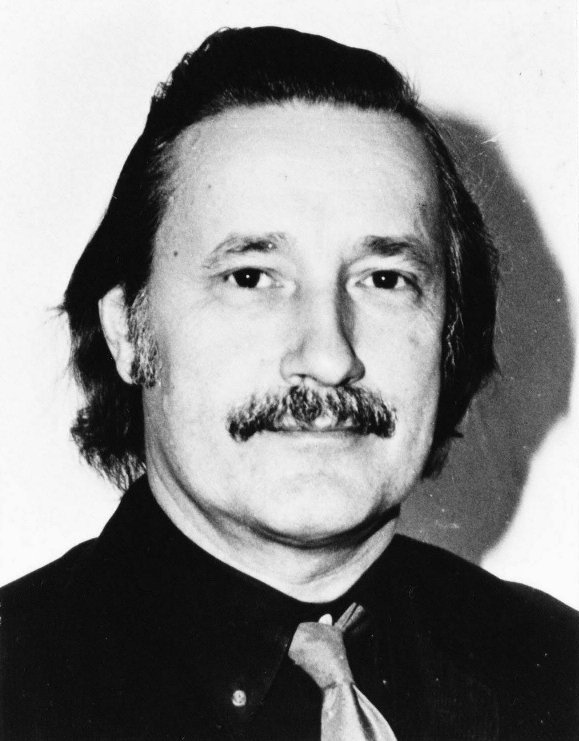
\includegraphics[angle=0,scale=0.2]{stratchey.jpg}
Кристофер Стретчи (Cristopher Stratchey, 1916-1975) был другом Алана Тьюринга, когда тот работал в Кембридже и Манчестере. Он известен тем, что написал программу для игры в шашки в 1951 году в Национальной Физической Лаборатории (National Physical Laboratory, NPL). Это, возможно, была первая иградющая программа на компьютере. Эта программа запускалась на машине Марк-1 манчестерского университета, так как имела намного больше памяти чем, например, машина ACE, которую спроектировал Алан Тьюринг. Для Марк-1 он также написал, первую программу для проигрывания простых мелодий, а именно десткой песенки Baa Baa Black Sheep.

Что касается языков программирования, К.Стретчи спроектировал CPL (Combined Programming Language), который назывался изначально Cambridge Programming language и после переезда в Лондон стал называться Combined. Также его называли Cristopher’s programming language. В этом языке были функции как сущности первого класса, а также было впервые введено понятие L-values --- выражений, которые вычисляются в место, где они хранятся. CPL никогда не был успешно реализован, были прототипы и в Лондоне, и в Кембридже, но язык был очень амбициозен и сложен для того времени, так что его компиляторы никогда не появились и пользователей у него не было. Однако, Мартин Ричардс написал выпускную работу про компилятор этого языка, и вскоре решил, что было бы хорошо несколько упростить язык CPl. Так появился Basic CPL (BCPL), компилятор которого был реализован. Это был очень упешный язык для реализации больших систем в конце 60х - начале 70х, который использовался, например, в компании Xerox Park. А в Bell Labs Кен Томпсон также начал использовать его и улучшать. Так появился язык В, который потом эволюционировал в С++.

\begin{verbatim}
CPL  =>  BCPL  =>  B  =>  C  =>  C++
\end{verbatim}

Также он ввёл понятие каррирования (currying). В середине 60х Стретчи написал очень важную работу, представленную на конференции в Копенгагене в 1967, которая называлась  “Фундаментальные понятия в языках программирования “ (Fundamental concepts in programming languages). В ней он описывал различные виды полиморфизма м первым описал параметрический полиморфизм. Так же он известен как создатель денотационной семантики Скотта-Стретчи (совместно с Дана Скотт (Dana Scott) в 1969, который предоставил математическое обоснование этой семантики, основанной на лямбда-исчислении). Также Стретчи первым дал формальное определение продолжений (continuations). Он пришел к идее разделения времени (time-sharing, 1958) правда в несколько урезанном виде. В 1960-64 он нанял Питера Лондина (Peter Lundin) как своего помощника, который работал в национальной Лаборатории физики и в National Research and Develpment Corporation в Лондоне, а с 1959 Лондин стал работать как независимый консультант. 

\begin{framed}
Вот что пишет Водсворт о Стретчи:

“Стретчи имел особое чутьё в тех случаях, когда что-то было сделано “правильно” -- в основном когда было достаточно просто и достаточно элегантно, что выглядеть интуитивно правильным -- и он презирал чересчур проработанные и умудренные методы который “кае какработали”. Его любимым принципом был такой: “Ты можешь затолкать на гору горошину носом, но это не будет являться правильным способом осуществления этого”. Я это называл “тестом Стретчи”.
”
\end{framed}
%\begin{framed}
%Бёрнсталл о Стретчи
%His elegance of Manor was accompanied by an elegance of thought and language which was a continual inspiration.
%\end{framed}

Питер Лондин (Peter Landin) % Фотка была выше
написал множество статей в 1960х годах.

“Механическое вычисление выражений” (The mechanical evaluation of expressions, 1964) которые ввело поянтие SECD машины. Это не была  первая абстрактная машина в мире, он использовал идеи сообщества программистов на языке ALGOL из города Мюнхен. 

В статье "Соответсвие между языком ALGOL60 и лямбда-нотацией Чёрча: части 1 и 2" (“A correspondence between ALGOL 60 and Chuch’s Lambda-notation: Part I and Part II”, 1965 год) он ввел понятие потоков (streams), которые являются особого рода методом для осуществления ввода-вывода.

В статье "Обобщение переходов и меток" ("A generalization of of Jumps and Labels”, 1965) он ввел понятие J-оператора, который является предшественником термина продолжение (continuation).

Статья "The next 700 programming languages" 1966 года, описывает ISWIM язык, который оказал влияние на ML \footnote{найти ещё про это}.

В статье "Programs and their Proofs: An algebraic Approach, в соавторстве с Burstall, 1969) он предвосхитил появление алгебраических типов данных. В предыдущих работах, например про ISWIM, использовались некоторые дополнительные лингвистические конструкции для описания структур данных, которые не являлись частью языка.

Pedagogical Algorithmic Language 
PAL: an implementation of ISWIM at MIT (Arthur Evans). Разработка этой штуки шла  в течение всех 60х.: в начале Стретчи приезжал пару раз в MIT в начале 60х, но дело не сдвигалось пока в 1967 году Лэндин не поработал в MIT в течение года, и тогда PAL превратился в некоторую реализацию ISWIM. 

\chapter{Робин Милнер}

Как и К.Стретчи, и П.Лэндин, он не начинал как ученый -- был школьным учителем, а перед тем как попасть в научную среду работал программистом на компанию Ferranti.
\begin{framed}
Из тьюринговской лекции:

“Идея того, чтобы машина доказывала теоремы используя логику, и идея того, чтобы ипользуя логику понимать что машина делала…. Эта двойственность вдохновляла меня потому, что очевидно это было не очень просто”
\end{framed}

Принципы, которыми следовали все эти люди
Стретчи, Лондин, Бёрсталл, Миленр ( и другие как Тони Хоар) основали Британскую традицию  в исследовании языков программирования

\begin{itemize}
 \item Осмысление важности фундаментальных основания и семантики в изучении вычислений и программирования
 \item Поиск ясности, строчгости и элегантности путём использования математическихз идей и подходов, в частности из логики и алгебры.
\end{itemize}

Эти принципы особенно прижились в сообществе Эдинбурга.
 
\section{Ситуация в Эдинбурге в конце 70х}
Р.Милнер на системой доказательства теорем LCF которая заработала в 1978-79х годах. В неё ML использовался как метаязык. (написать ещё используя ссылку ). Осенью 1978 в Эдинбург приезжает Лука Карделли как grad student для получения Ph,D, . Роб Бёрсталл и Дэйв МакКуин работали на языком программирования HOPE -- чистым языком программирвоания, первым языков с алгебраическими типами данных.  Хотя за год до этого Бёрсталл сделал игрушечный язык программирвоания MPL, где АДТ таки были, но немного по-ругому к типам добавлялись их конструкторы.  
В Эдинбурге было два подсообщества. Бёрсталовское было в Школе ИИ (School of Artificial Intelligence) на какой-то там площади. Милнеровское было в King’s Science Building на три миле южнее. И они сделали существенный барьер между этими двумя группами -- не так просто было сходить туда-сюда. Решение нашлось в лице Bob Boyer memorial society. Тот получал Ph.D. в Школее ИИ. И когда он покинул Эдинбург, его работу как организатора начали выполнять другие люди: народ собирался по вечерам дома у Робина Миленра  или в гостиной у кого-нибдуь друго.го. И это сближало два   сообщества. В конце концов посетители стали ядром Лаборатории Основ Информатики (Laboratory for Foundations of Computer Science, LFCS), хотя даборатория формально не сущестовала до 1986 года.  Кроме Робина Милнера, Бёрсталла и Плоткина этим занимался Мэтью Хеннеси .

Связи в  те времена 

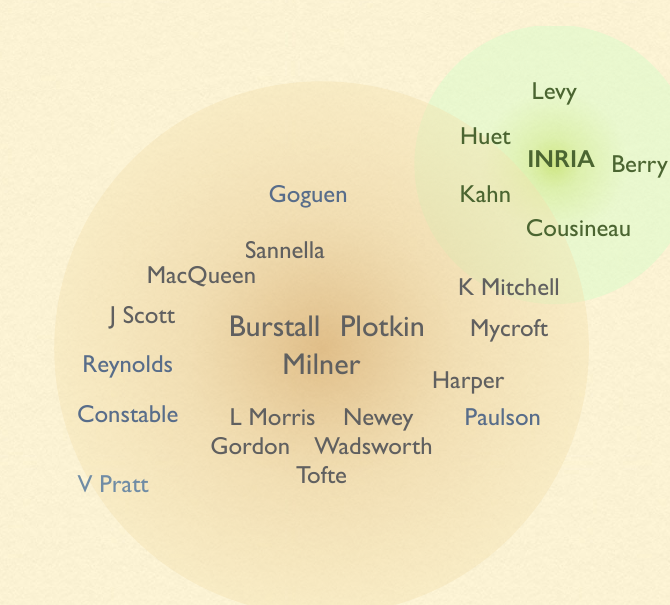
\includegraphics[angle=0,scale=0.585]{two_circles.png}

Как бы ценр вселенной. Три ключевых фигуры, а также первое поколение их учеников. Другое сообщество было в INRIA. Постоянные разъезды с финансированием за счет государства.

LCF/ML aka DEC10 ML (25:16---...)
Встраивался в систему LCF как метаязык
Включал в себя объектный язык PPLAMBDA (который использовался как оописание LCF логики Скотта). 
Термы, формулы, теоремы 
Ключевой особенностью было то, что теоремы были абстрактными типами и конструирование термов могло происзожить только путём применения правил вывода.
Quotation/antiquotation в синтаксисе
Тактики и тактики высшего порядка, которые комбинировали другие тактики -- дляэтого им был нужен функциональный язык пограммирования. Также был нужен сильно типизированный язык программирования, чтобы быть уверенными, что не существует обходного подхода для создания теорем

Основные свойства LCF/ML
\begin{itemize}
  \item Основан на ICWIM
  \item Вывод типов Через милнеровский let-polymorphism,
  \item Абстрактные типы данных (через ключевое слово abstype).
  \item Тип-сумма и тип-произведение (t1+t2, t1\#t2)
  \item Мутабельные переменные через объявление letref (с хитрыми типами типизации)
  \item Вложенные кортежи и шаблоны для байндинга списков.
  \item Условные циклы
  \item Поддержка ошибочных ситуаций путём передачи строк(которые назывались токенами). Простые ловушки, условные и зацикливающиеся 
\end{itemize}


 Компилятор был изначально написан на LISP (вначале на диалекте Standford, потом Rutgers). Код с ML транслировался в LISP и интерпретировался, поэтому был медленным. Парсер был онсован на приоритетном парсере Вона Пратта (Vaugnan Pratt) который имел ту особенность, что функциии-парсер прикреплялись к отдельно взятым символам, когда было бы более естественно использовать разные парсеры для одного и того же символа в зависимости от контекста. Такоим образом получалось, что если запятая использовалась для разделения элементов кортежа, то её нельзя было использовать для разделения элементов списка, а если точка с запятой использовалась для разделения элементов списка, то для оператора следования нужно было использовать удвоенную точку с запятой, и т.д.

VAX ML (aka Cardelli ML)
В 1980 начинает работу на собственным диалектом ML его компилятором. Всё реализовывает сяна паскале. Со сборщиком мусра. К 1981 году закончил это дело.

Нововведения
\begin{itemize}
 \item Именованные структуры и варианты -- на основе Плоткинских лекций по теории доменов.  До этого они не объявлялись явно перед использованием.
\item Declaration combinators
\item Ref type operator вместо конструкции letref. А также правила вывода для него, ref, !, :=.
\item Stream I/O
\item Базовая поддержка модулей (раздельная компиляция

\end{itemize}


Declaratoin combinators:
and одновременно;
enc -- последовательно (enclosing)  ⇒ d1;d2
Ins -- local (inside) ⇒ local d1 in d2 end;
Rec -- recusive
With -- для особой формы абстрактных типов (объявления вида with t ⇔ ty)

\chapter{VAX ML compiler (Эдинбург, 1980-1982)}
Запускался под операционной системой VAX/VMS.
ЙЦеликом на паскале, включая рантайм
Весь код компилровался в FAM (Functional abstract Machine).
Генерировала код для VAX машины из FAM кода.
Экспорт/импорт модлей на лету.

Продовалась пользователям с 1981

Роль
Показало, что ML может использоваться как язык общегоназначения и имеет эффективную реализацию. 
Привело к росту количества диалектов ML. Привело к предложению от Р.Милнера “стандартизовать” ML (Standart ML, SML, April 1983).
Непосредсвенный предшественник SML
Тестовая площадка для ранних экспериментов над дизайном SML.

 Встречи по дизайну: апрель 1983, июнь 1984, май 1985. Так получилось что ольшое количество людей собиралось в Эдинбурге. В апреле Р.Милнер презентовал первый предложение по станджартизации (ссылка тут). 

Первая встреча а апреле 1983
Организовал всё Бернард Суфрин. Р.Милнер написал первое продложение  собирая идеи из LCF/ML, VAX ML и HOPE. Всё проходил о в гостиной Милнера

physical participants
Rod Burstall, Luca Cardelli, Guy Cousineau, Mike Gordon, David MacQueen, Robin Milner, Kevin Mitchell, Alan Mycroft, Larry Paulson, David Rydeheard, Don Sannella, John Scott, Brian Monahan, Stefan Sokolowski

virtual participants
Gerard Huet, Peter Mosses, David Schmidt

Название Р.Милнер выбрал сам, чтобы надеясь предотвратить длительные споры о дизайне языка , хотя это оказалась ошибкой, поэтому что такое амбиционое имя в некотором смысле приклеилось

Первые фичи из драфта
Формы объявления типов данных, конструкторы в паттернах.
Без записей и вариантов (в смысле VAX ML)
Функциональные выражения с клаузами :  fun v1. e1 | ... | vn. en
monomorphic references and equality
“local” declaration instead of Cardelli’s “ins” operatorЖ
Механизм обработки ошибок (escape) с токеном и единая форма обработки (trap) для этого:
e1 trap v1. e1 | ... | vn. En. Но исключения могли в себе нести только строки.


Further drafts (for Core SML)
4/83: Changes to proposal for Standard ML, Milner
6/83: A Proposal for Standard ML (second draft), Milner (49 pages)
11/83: A Proposal for Standard ML, Milner (27 pages) [“final”]
6/84: Record of the Standard ML Meeting, Edinburgh, 6-8 June 1984
MacQueen and Milner
7/84: Standard ML - The Core Language, Milner [changes summary]
7/84: The Standard ML Core Language, Milner [LFP 84 draft?]
10/84: The Standard ML Core Language, Milner
6/85: Report on the Standard ML Meeting, Edinburgh, May 23-25, 1985, Harper
9/85: The Standard ML Core Language (Revised), Robin Milner

В те времена ещё не было email и ARPANET, поэтому вся переписка велась через почтовое сообщение. Постепенно спецификация стандарта менялась, наращивая небольшие изменения. В июне 1985голюди собрались во второй раз, называя это уже ML Workshop (первый из них).

Так же были предложения по спецификации  других частей языка.

Other Design Drafts - I/O and Modules
Stream I/O:
12/83: Stream Input/Output, Cardelli [Polymorphism 3,1]
2/85: Proposal for I/O in Standard ML, K. Mitchell and Milner
6/85: Standard ML Input/Output, Harper [ML Workshop 85]
Modules:
8/83: Modules for Standard ML, MacQueen [preliminary, incomplete draft]
8/84: Modules for Standard ML, MacQueen [LFP 84, Polymorphism]
10/85: Modules for Standard ML, MacQueen [final draft before Definition]




The Definition of Standard ML (SML ’90)
Work on the formal definition started sometime in 1986. Three drafts of
the formal definition of the entire language appeared as Edinburgh LFCS
Tech Reports written by Milner, Harper, and Mads Tofte (Robin’s student).
8/87: The Semantics of Standard ML, Version I
8/88: The Definition of Standard ML, Version 2
5/89: The Definition of Standard ML, Version 3
The Definition was eventually published in 1990 by MIT Press.

Одно из самых важных нововведений, которое было предложено не в самом начале, была поддержка исключений как расширяемых типов данных. Язык был расширен конструкторамиисключений и паттер-матчингом исключений в их обработчике. 

Three Early Implementations

Cardelli’s VAX ML => “subStandard ML”
Early Standard ML features added in 1983-84
Edinburgh ML => Edinburgh SML
Kevin Mitchell, Alan Mycroft, John Scott and Bob Harper (Взяли Cardelli’s ML и переписали компилятор на нём (bootstrap))
PolyML by Dave Matthews at Cambridge
Standard ML front end built for his Poly compiler

Более поздние реализации:
\begin{itemize}
 \item Standart ML of New Jersey
 \item MLKit (with Regions)
 \item Moscow ML
 \item MLton
\end{itemize}

\subsection{ Главные идеи в  Standard ML ‘90}
Let-полиморфизм, type inference, principal types: Newman (1943!), Curry (1969), Hindley (1969), Milner
Algebraic data types, with clausal functions, case analysis via pattern-matching [from Hope]
Modules with signatures, functors, sharing specifications, and generative structures (“strong structure sharing”) структуры  с  некоторой статической уникальной идентичностью, которые  можно было сравнивать, т.е. На этапе компиляции можно проверить, что структуры идентичны (равны). Там получалась очень сложна семантика, потому оно не стало особо популярно
Exceptions as an extensible data type
Support for mutable variable (a.k.a. ref types) using понятие “imperative type variables” что привело к большим пролблемам. Большое количестов статей на тему того как улучшить данных подход и почему от него стоит отказаться.

Эволюция алгебраических типов данных.
Исторически дизайн заимстован в Лондина. 
\begin{enumerate}
\item Неформальные описания данных, использованные в ISWIM.
\item Формальное развитие этих методов в работе Люндина и Бёрсталла “Programs and Their Proofs: An Algebraic Approach” (полу \item формаьно описаны)
\item “Игрушечный” язык Бёрсталла NPL
\item В Языке HOPE более-менее полно софрмировались и перекочевали оттуда в Standart ML.
\end{enumerate}



Картинка
\begin{verbatim}
datatype AE = ID of identifier
            | LAMBDA of {bv: identifier, body : AE}
            | COMB of {rator : AE, rand : AE}
\end{verbatim}

\subsection{Ошибки в процессе дизайна}
“Заморажвагие” формального описания языка в виде книги: если язык программирования реализуется и начинает использоваться, то его описание необоходимо поддерживать, а также (весьма осоторожно) позволять ему изменяться. Описание должно быть открытым, но при этом очень аккуратно поддерживаемым.
Это связано со степенью участия Милнера в проекте. Он был весьма занятым человеком, его основными проектами в то время были CCS и пи-исчисление. Т.е. Ему хотелось дойти до состояния, когда он может передать рукопись в издателсттво MIT  и перстать думать об этом проекте. Для своих целей он не планировал реализовывать поддерживать и даже использовать этот языка. Однако, если язык будут реализоваывать поддерживать и ииспользовать, то его описание должно поддерживаться тоже. В те времена не сущестоввало WWW, так что не было варианта выложить описане в онлайн.
Выпущенная книга про SML’90 имела очень короткое (2-3 странице) приложение про “основы”, что было скорее про стандарную библиотеку, встроенные типы и функции. Их список был очень короткий и состоял только из 43х пунктов. Т.о. Каждый кто реализовывал SML должен был расширять этот перечень, и каждая реализация расширяла этот список несовместимым друг с другом способом. Процесс устанаканивая занял довольно длительное время, то тех пор как Reppy и Gasner не взялись  за это и не создали “SML Basis Library” однако их работа вышла в сает спустя несколько лет после SML‘97.

\subsection{Развитие языка в 1990е годы}
SML;97 переработанное описать Standart ML
В 1997 году инсттитут Ньютона(Isaac Newton Institute for Mathematical Sciences), а именно программа по исследованию семантики вычислений собрала Мильнера, Харпера, Тофте и МакКуина в Кембридже, где они начали работу над пересмотру описания языка Standart ML. Значимые исменения 

\begin{itemize}
 \item Сокращения типов в сигнатурах (SML/NJ 0.93; Harper, Leroy POPL 94)
\item Opaque signature matching
\item Weak structure sharing (structure sharing implies only type sharing) 
\item Value polymorhism (eliminataion of imperative type variables, a.k.a. Value restriction)
\item Replication of datatypes.
\end{itemize}
Также хотели выкинуть equality types, но Милнер застеснялся.

\subsection{ML2000}
Серия встреч между 1993 и 2000 годами была посвещена идеи создания ML “следующего поколения”,  но консенсус так и не был пройден в основном из-за не согласия участников по поводу добавления объектно-ориентированных возможностей в язык.
В то время уже сощестовали языки такие как OCaml со своейсобственной реализацией объектов, а также язык Moby за авторством Reppy и Fisher’a. 
Статья Principles and Preliminary Design of ML2000. 


\section{A History of OCaml}
“Caml” was originally an acronym for Categorical Abstract Machine Language. It was a pun on CAM, the Categorical Abstract Machine, and ML, the family of programming languages to which Caml belongs. The name Caml has remained throughout the evolution of the language, even though the present implementation has no relation with the CAM.
Caml was first designed and implemented by Inria's Formel team, headed by Gérard Huet. Its development continued within the Cristal team, and its current successor, Gallium.
\subsection{The Origin}
The Formel team became interested in the ML language in 1980–81. ML was the meta-language of the Edinburgh version of the LCF proof assistant, both designed by Robin Milner. It was implemented by a kind of interpreter written in Lisp by Mike Gordon, Robin Milner and Christopher Wadsworth. LCF itself was written partly in ML and partly in Lisp. In order to be able to use the LCF proof assistant on the various systems in use at Formel at that time (Multics, Berkeley Unix on Vax, Symbolics), Gérard Huet decided to make the ML implementation compatible with various Lisp compilers (MacLisp, FranzLisp, LeLisp, ZetaLisp). This work involved Guy Cousineau and Larry Paulson. The performance of the ML implementation was improved by the addition of a compiler.

Guy Cousineau also added algebraic data types and pattern-matching, following ideas from Robin Milner, which he in turn had borrowed from Hope, a programming language designed by Rod Burstall and Dave McQueen. At some point, this implementation was called Le\_ML, a name that did not survive. It was used by Larry Paulson to develop Cambridge LCF and by Mike Gordon for the first version of HOL, as recalled in Gordon's short history of HOL.
Around 1984, three events motivated us to get even more involved in the development of ML:
In Edinburgh, Luca Cardelli developed a much faster implementation of ML using his Functional Abstract Machine (FAM). He also designed his own version of the language, known at that time as Cardelli's ML.
Robin Milner thought it was a good moment to propose a new definition of ML in order to avoid divergence between various implementations. He defined the core Standard ML language, which was later complemented by a module system designed by Dave McQueen.

At the same time, Pierre-Louis Curien developed a calculus of categorical combinators, as well as a correspondence between lambda-calculus and categorical combinators, which, as noticed by Guy Cousineau, could be seen as a compilation technique for ML. Indeed, it was quite close to the original implementation technique of Edinburgh ML, but could be described, proved correct, and optimized in a simple way. This led to the definition of the Categorical Abstract Machine (CAM).
This urged Guy Cousineau to develop a new implementation of ML, based on the CAM. However, the language that we ended up implementing was not Standard ML, but... Caml. Why? Our main reason for developing Caml was to use it for software development inside Formel. Indeed, it was used for developing the Coq system, which, following Thierry Coquand's thesis in 1985, became the team's main aim. We were reluctant to adopt a standard that could later prevent us from adapting the language to our programming needs. In particular, Philippe Le Chenadec and Michel Mauny developed syntax manipulation tools that appeared useful and were incorporated into Caml. Synchronizing with the Standard ML team before adopting the language modifications that seemed useful to us would have introduced too much delay in our work. Furthermore, our philosophy was in conflict with that of a “standard” language, which is not supposed to evolve too quickly. We did incorporate into Caml most of the improvements brought by Standard ML over Edinburgh ML.

\subsection{The First Implementation}
The first implementation of Caml appeared in 1987 and was further developed until 1992. It was created mainly by Ascander Suarez. After Ascander left in 1988, Pierre Weis and Michel Mauny, carried on with the development and maintenance of the system. This implementation compiled Caml down to LLM3,
the virtual machine of the Le\_Lisp system. Guy Cousineau modestly recalls: “I must admit that when the Caml development started, my experience with programming language implementation was very limited. Relying on the LLM3 abstract machine and on the Le\_Lisp memory allocation and garbage collection system saved a lot of work but could not lead to high efficiency. The CAM model led to fast closure construction and good environment sharing but was poor at environment access and made optimizations difficult. It also potentially introduced memory leaks, since useless values were kept inside closures. Also, I had not realized that it was more important to have good performance on non-functional programs than on very functional ones. Above all, I had overlooked the importance of portability and openness. In spite of these inadequacies, for which I am initially responsible, Ascander, Pierre and Michel did quite a nice piece of work.”
\subsection{Caml Light}
In 1990 and 1991, Xavier Leroy designed a completely new implementation of Caml, based on a bytecode interpreter written in C. Damien Doligez provided an excellent memory management system. This new implementation, known as Caml Light, was highly portable and easily ran on small desktop machines such as Macs and PCs. It replaced the old Caml implementation and highly helped promote the use of Caml in education and in research teams. Its support for data streams and its parsing facilities, due to Michel Mauny, were issued from a continued effort of the Formel team to promote syntax manipulation tools.
\subsection{Caml Special Light}
In 1995, Xavier Leroy released Caml Special Light, which improved over Caml Light in several ways. First, an optimizing native-code compiler was added to the bytecode compiler. This native-code compiler matched or exceeded the performances of the best existing compilers for functional languages, and enabled Caml to be more competitive performance-wise with mainstream imperative programming languages such as C++. Second, Caml Special Light offered a high-level module system, designed by Xavier Leroy and inspired by the module system of Standard ML. This module system provides powerful abstraction and parametrization facilities for programming in the large.
\subsection{Objective Caml}
Type systems and type inference for object-oriented programming has been a hot area of research since the early 1990's. Didier Rémy, later joined by Jérôme Vouillon, designed an elegant and highly expressive type system for objects and classes. This design was integrated and implemented within Caml Special Light, leading to the Objective Caml language and implementation, first released in 1996 and renamed to OCaml in 2011. Objective Caml was the first language to combine the full power of object-oriented programming with ML-style static typing and type inference. It supports many advanced OO programming idioms (type-parametric classes, binary methods, mytype specialization) in a statically type-safe way, while these idioms cause unsoundness or require run-time type checks in other OO languages such as C++ and Java.

In 2000, Jacques Garrigue extended Objective Caml with several new features, which he had been experimenting with for a few years in the Objective Label dialect of Objective Caml. Among these features were polymorphic methods, labeled and optional function arguments, and polymorphic variants.
The rise of OCaml
Since the late 1990's, OCaml has been steadily gaining in popularity and attracted a significant user base. In addition to impressive programs developed in OCaml, the user community also contributed many high-quality libraries, frameworks and tools in areas ranging from graphical user interfaces and database bindings to Web and network programming, cross-language interoperability and static program analysis. In parallel, the core OCaml development team actively maintains the base system, improving the quality of the implementation and porting it to the latest architectures and systems. As lead developer of OCaml, Chair of the Caml Consortium and Owner of OCaml.org, Xavier is considered to be benevolent dictator for life (BDFL) of the OCaml language.
Some Close Relatives
In addition to these mainstream versions of Caml, one should mention many related compilers. Michel Mauny and Daniel de Rauglaudre designed Chamau, which offers unique syntax manipulation facilities which are now offered in the Camlp4 pre-processor for OCaml.
Manuel Serrano and Pierre Weis created BIGLOO. Régis Cridlig made Camlot. Jean Goubault-Larrecq wrote HimML, which features implicit hash-consing and efficient operations on sets and maps. Emmanuel Chailloux published CeML. In the Para team, Francis Dupont implemented Caml for parallel machines, while Luc Maranget built Gaml, a compiler for a lazy functional programming language.
\subsection{Final Quote}
In 1996, Guy Cousineau wrote: “Certainly, the history of Caml could have been more linear. However, through trial and error, a capacity for producing high performance, portable, and flexible functional programming language implementations has emerged in France.”

\newpage
\begin{thebibliography}{9}
  \bibitem{hilGeo}
    Д. Гильберт. Основания геометрии, перевод с немецкого под редакцией А.В.Васильева,
    Л., "Сеятель", 1923 — 152 с.
  \bibitem{kushner}
    Б.А. Кушнер. Лекции по конструктивному математическому анализу. — М.: Наука, 1973. — 447 с.
  \bibitem{taran}
    К. Таран. Метод применения Теории Типов Мартина-Лёфа для верификации программных систем.
    Дипломная работа, кафедра СП, СПбГУ, 2014.
  
  \bibitem{baren}
    H. Barendregt. Lambda Calculi with Types, Handbook of Logic in Computer Science, Volume II, Oxford University Press, 1991.
  \bibitem{coc}
    T. Coquand, G. Huet. The Calculus of Constructions, Information and Computation 76 (2–3), 1988.
  \bibitem{curry}
    H.B. Curry, R. Feys. Craig, William, ed., Combinatory Logic Vol. I, Amsterdam: North-Holland, 1958. p. 9E.
  \bibitem{gont}
    G. Georges. Formal Proof—The Four-Color Theorem, Notices of the American Mathematical Society 55 (11): 1382–1393, 2008.
  \bibitem{Hott}
    Homotopy Type Theory: Univalent Foundations of Mathematics. — Princeton: Institute for Advanced Study, 2013.
  \bibitem{howard}
    W.A. Howard. The formulae-as-types notion of construction, in Seldin, Jonathan P.; Hindley, J. Roger, To H.B. Curry: Essays on Combinatory Logic, Lambda Calculus and Formalism, Boston, MA: Academic Press, 1980 (original paper 1969). pp. 479–490
  \bibitem{makkai}
 M. Makkai. First Order Logic with Dependent Sorts, with Applications to Category Theory, 1995.
  \bibitem{progML}
    B. Nordström, K. Petersson, J. M. Smith. Programming in Martin-Löf's Type Theory. Oxford University Press, 1990.
  \bibitem{norell}
    U. Norell. Towards a practical programming language based on dependent type theory. PhD Thesis. Chalmers University of Technology, 2007.
  \bibitem{itt} P. Martin-Löf. Intuitionistic type theory,
    Studies in proof theory: Lecture notes (1), Giovanni Sambin, Bibliopolis, 1984.
  \bibitem{presburger}
    M. Presburger. Über die Vollständigkeit eines gewissen Systems der Arithmetik ganzer Zahlen, in welchem die Addition als einzige Operation hervortritt. Comptes Rendus du I congrès de Mathématiciens des Pays Slaves, 1929.  Warszawa. p. 92-101.
  \bibitem{russel1}
    A.N. Whitehead, B. Russell Principia mathematica 1 (1 ed.), Cambridge: Cambridge University Press, 1910.
  \bibitem{russel2}
    A.N. Whitehead, B. Russell. Principia mathematica 2 (1 ed.), Cambridge: Cambridge University Press, 1912.
  \bibitem{russel3}
    A.N. Whitehead, B. Russell. Principia mathematica 3 (1 ed.), Cambridge: Cambridge University Press, 1915.
  \bibitem{zhao}
     L. Zhaohui. Computation and reasoning: a type theory for computer science. Oxford University Press, Inc., 1994.
\end{thebibliography}

\end{document}
